\documentclass[12pt]{article}
\usepackage[top=1in, bottom=1in, left=1in, right=1in]{geometry}

\usepackage{setspace}
\onehalfspacing

\usepackage{amssymb}
%% The amsthm package provides extended theorem environments
\usepackage{amsthm}
\usepackage{epsfig}
\usepackage{times}
\renewcommand{\ttdefault}{cmtt}
\usepackage{amsmath}
\usepackage{graphicx} % for graphics files

% Draw figures yourself
\usepackage{tikz} 

% writing elements
\usepackage{mhchem}

% The float package HAS to load before hyperref
\usepackage{float} % for psuedocode formatting
\usepackage{xspace}

% from Denovo Methods Manual
\usepackage{mathrsfs}
\usepackage[mathcal]{euscript}
\usepackage{color}
\usepackage{array}

\usepackage[pdftex]{hyperref}
\usepackage[parfill]{parskip}

% math syntax
\newcommand{\nth}{n\ensuremath{^{\text{th}}} }
\newcommand{\ve}[1]{\ensuremath{\mathbf{#1}}}
\newcommand{\Macro}{\ensuremath{\Sigma}}
\newcommand{\rvec}{\ensuremath{\vec{r}}}
\newcommand{\vecr}{\ensuremath{\vec{r}}}
\newcommand{\omvec}{\ensuremath{\hat{\Omega}}}
\newcommand{\vOmega}{\ensuremath{\hat{\Omega}}}
\newcommand{\sigs}{\ensuremath{\Sigma_s(\rvec,E'\rightarrow E,\omvec'\rightarrow\omvec)}}
\newcommand{\el}{\ensuremath{\ell}}
\newcommand{\sigso}{\ensuremath{\Sigma_{s,0}}}
\newcommand{\sigsi}{\ensuremath{\Sigma_{s,1}}}
%---------------------------------------------------------------------------
%---------------------------------------------------------------------------
\begin{document}
\begin{center}
{\bf NE 250, F15\\
September 28, 2015 
}
\end{center}

Public service announcements: 
\begin{itemize}
\item Grad student mental health resources: \href{http://www.uhs.berkeley.edu/students/counseling/cps.shtml}{http://www.uhs.berkeley.edu/students/counseling/cps.shtml}
\item Sexual assault support on campus: \href{http://survivorsupport.berkeley.edu/}{http://survivorsupport.berkeley.edu/}
\item Documentary \textit{The Hunting Ground} (\href{http://www.thehuntinggroundfilm.com/}{http://www.thehuntinggroundfilm.com/}) and Lady Gaga's corresponding music video about sexual assault on college campuses (trigger warning): \href{https://www.youtube.com/watch?v=ZmWBrN7QV6Y}{https://www.youtube.com/watch?v=ZmWBrN7QV6Y}
\end{itemize}

We won't do the last problem of the homework assignment this class. It turns out Max did a Serpent tutorial before assigning Serpent problems, so it only seems fair I do the same. If you've already done it it will be on the next assignment, but for the rest of you we will have a Serpent tutorial on Monday, October 5.

Also, I am going to update the homework deadline to 3 pm (rather than 5).
You can turn it in to Kelly on Fridays when it's due (can leave it on her desk in 3115 Etcheverry if she's not there).

--------------------------------------------\\
Last time we talked about solving linear differential equations. 
Given $M$ as a non-homogenous differential operator of order \emph{n} on a differential equation
%
\begin{equation*}
M\phi(x) = f(x) \:.
\end{equation*}
%
One solution method is \textit{variation of constants / parameters}, where we break the solution into homogeneous and particular portions.
\begin{align*}
\phi_{i,h}(x),  \:i &= 1,\dotsc, n \:\text{ independent solutions} \\
\phi_{part}(x) &= \sum_{i=1}^n c_i\phi_{i,h}(x)\\
\sum_{i=1}^n c'_i(x) \phi^{(j)}_{i,h}(x) &= 0, \quad j = 0, \dots, n-2 \\
\sum_{i=1}^n c_i'\phi^{(n-1)}_{i,h}(x) &= \frac{f(x)}{a_0(x)} \\
c_i(x)& = \int dx\:c_i'(x) \:.
\end{align*}


----------------------------------------\\
For a plane source in an infinite medium:
\begin{equation*}
\frac{d^2\phi(x)}{dx^2} - \frac{1}{L^2}\phi(x) = -\frac{S\delta(x)}{D}
\end{equation*}

Homogeneous problem: $\frac{d^2\phi}{dx^2} - \frac{1}{L^2}\phi(x)=0,\phi_1(x)=e^{-x/L},\phi_2(x)=e^{x/L}$

\begin{equation*}
e^{-x/L}c_1'(x) + e^{x/L}c_2'(x) = 0
\end{equation*}

\begin{equation*}
-\frac{e^{-x/L}}{L}c_1'(x) + \frac{e^{x/L}}{L}c_2'(x) = -\frac{S}{D}\delta(x)
\end{equation*}

\begin{equation*}
\phi_{part}(x) = c_1(x)\phi_1(x) + c_2(x)\phi_2(x)
\end{equation*}

\begin{equation*}
c_1'(x) = \frac{SL}{2D}\delta(x)e^{x/L}
\end{equation*}

\begin{equation*}
c_2'(x) = -\frac{SL}{2D}\delta(x)e^{-x/L}
\end{equation*}

\begin{equation*}
c_1(x) = \int_{-\infty}^x dx\frac{SL}{2D}\delta(x)e^{x/L} = \frac{SL}{2D}H(x),
\text{ where $H(x)$ is the Heaviside step function}
\end{equation*}

\begin{equation*}
  H(x)=\begin{cases}
    1, & x > 0 \\
    \tfrac{1}{2}, & x = 0 \\
    0, & x > 0
  \end{cases}
\end{equation*}

\begin{equation*}
c_2(x) = \int_{-\infty}^x dx\frac{-SL}{2D}\delta(x)e^{-x/L} = -\frac{SL}{2D}H(x),
\end{equation*}

\begin{equation*}
\phi(x) = A_1\phi_1(x) + A_2\phi_2(x) + c_1(x)\phi_1(x) + c_2(x)\phi_2(x)
\end{equation*}

\begin{equation*}
\phi(x) = \left(A_1 + \frac{SL}{2D}H(x)\right)e^{-x/L} + \left(A_2 - \frac{SL}{2D}H(x)\right)e^{x/L}
\end{equation*}

Boundary conditions:
\vspace{-5 mm}
\begin{gather*}
\lim\limits_{x\to\infty}|\phi(x)\ < \infty \rightarrow A_2 = \frac{SL}{2D} \\
\lim\limits_{x\to-\infty}|\phi(x)\ < \infty \rightarrow A_1 = 0
\end{gather*}

\begin{equation*}
\phi(x) = \frac{SL}{2D}H(x)e^{-x/L} + \frac{SL}{2D}[1-H(x)]e^{x/L} = \frac{SL}{2D}e^{-|x|/L}
\end{equation*}

%2013-10-8
%--------------------------------------------------------------------
Other solution methods include the use of Green's function and the eigenfunction expansion method.

\underline{Green's function}

We will create a solution that looks like
\[M\phi_g(x) = \delta(x-x')\]
and will call $\phi_g(x) = G(x,x')$ the Green's function for operator $M$. Then
\[\phi(x) = \int dx' \: G(x,x') f(x')\:.\]

%For our problem
%%
%\begin{align*}
%\nabla\cdot[D(\rvec)\nabla\phi(\rvec)] &- \Sigma_a\phi(\vecr) = -S(\rvec)\:, \quad \forall \vecr \in V \\
%\phi(\rvec) &= 0\:, \quad \forall \vecr \in S \equiv \partial V
%\end{align*}
%
%Then, consider a unit source at $\rvec'$.
%$G(\rvec,\rvec') = $ flux at $\rvec$ due to a unit source $\rvec'$ and
%%
%\begin{align*}
%\nabla\cdot[D(\rvec)\nabla G(\rvec,\rvec')] &- \Sigma_a G(\rvec,\rvec') = -\delta(\rvec - \rvec')\:, \quad
%\forall \rvec \in V \\
%G(\rvec,\rvec') &= 0\:, \quad \forall \vecr \in S \equiv \partial V \:.
%\end{align*}
%%
%Now, 
%\begin{multline*}
%\int_V dV \left\{\nabla\cdot[D(\rvec)\nabla\phi(\rvec)]G(\rvec,\rvec') - 
%\nabla\cdot[D(\rvec)\nabla G(\rvec,\rvec')]\phi(\rvec)\right\} \\
%= \int_S dS \hat{e}_s\cdot D(\rvec)[\nabla\phi(\rvec)\times G(\rvec,\rvec') - 
%\phi(\rvec)\nabla G(\rvec,\rvec')] = 0
%\end{multline*}
%
%\begin{equation*}
%\int_V dV \left\{S(\rvec)G(\rvec,\rvec') - \delta(\rvec-\rvec')\phi(\rvec)\right\} = 0
%\end{equation*}
%
%\begin{equation*}
%\phi(\rvec') = \int_V dVS(\rvec)G(\rvec,\rvec')
%\end{equation*}
%
%\begin{equation*}
%\phi(\rvec) = \int_V dVS(\rvec')G(\rvec',\rvec)
%\end{equation*}
%
%Green's function (``kernel"): $G(\rvec,\rvec') = G(\rvec',\rvec)$
%
%
%The challenge is: how do we determine Green's function?


Consider a plane source in an infinite medium.
%
\begin{align*}
\frac{d^2\phi(x)}{dx^2} &- \frac{1}{L^2}\phi(x) = -\frac{S}{D}\delta(x)\\
&\lim\limits_{x\to\pm\infty}\phi(x) = \infty\\
\frac{d^2 G(x,x')}{dx^2} &- \frac{1}{L^2}G(x,x') = -\frac{\delta(x-x')}{D}\\
&\lim\limits_{x\to\pm\infty}G(x,x') = 0
\end{align*}

Using variation of constants to solve the Green's function part:
%
\begin{equation*}
G(x,x') = \frac{L}{2D}H(x-x')e^{-(x-x')/L} + \frac{L}{2D}[1-H(x-x')]e^{(x-x')/L}
\end{equation*}

\begin{align*}
\phi(x) &= \int_{-\infty}^{\infty}dx'G(x,x')\delta(x')S\\
\phi(x) &= \frac{SL}{2D}e^{-|x|/L}
\end{align*}

%--------------------------------------------------------------------
%--------------------------------------------------------------------
-------------------------------------------------\\
I've been looking ahead, and I'd like to change the course to be much more transport oriented than diffusion oriented. 
This means the material would come much more out of Bell and Glasstone (freely available online) and Lewis and Miller (not) than Duderstadt. 
Would that be okay for everyone?
I think it will be way more interesting. 

With that in mind, here's an update of the TE, where I will use $\psi(\vec{r}, E, \vOmega, t)$ for angular neutron flux.
%
\begin{align*}
\frac{1}{v} \frac{d \psi}{dt} &+ \vOmega \cdot \nabla \psi(\vec{r}, E, \vOmega, t) + \Sigma_t \psi(\vec{r}, E, \vOmega, t) = \int_{4 \pi} d\vOmega' \int_0^{\infty} dE' \: \Sigma_s(E', \vOmega' \rightarrow E, \vOmega) \psi(\vec{r}, E', \vOmega', t)\\
 +& \frac{\chi(E)}{4 \pi}\int_0^{\infty} dE' \: \nu(E') \Sigma_f(E') \int_{4 \pi} d\vOmega' \:\psi(\vec{r}, E', \vOmega', t + S(\vec{r}, E, \vOmega, t)
\end{align*}

For generality (and because it can be tricky), I want to cover the \underline{streaming term in curvilinear coordinates}.
$\vOmega \cdot \nabla$ is the derivative of angular flux along the direction of motion $\vOmega$. (See Figure~\ref{fig:cart-coord}).
%
\begin{figure}[h!]
    \begin{center}
    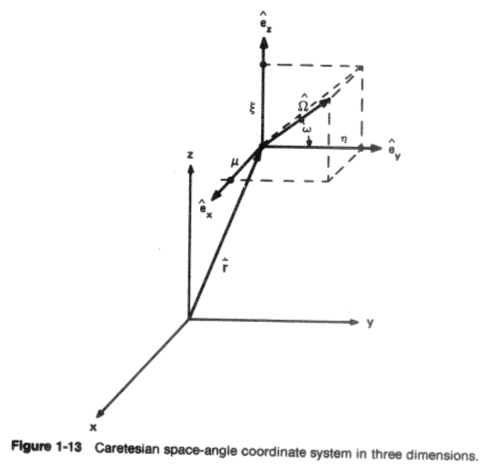
\includegraphics[keepaspectratio, width = 4 in]{../figs/cartesian-coords}
    \end{center}   
    \caption{Cartesian: L\&M Chp.\ 1}
    \label{fig:cart-coord}
\end{figure}
%
\begin{align*}
\vOmega &= \hat{e}_1 \cos(\theta) + \hat{e}_2 \cos(\gamma) + \hat{e}_3 \cos(\chi) \\
\nabla &= \hat{e}_1 \underbrace{\mathcal{D}_1}_{\text{derivative in direction }\hat{e}_1} + \hat{e}_2 \mathcal{D}_2 + \hat{e}_3 \mathcal{D}_3\\
&= \hat{e}_1 \frac{d}{dx} + \hat{e}_2 \frac{d}{dy} + \hat{e}_3 \frac{d}{dz} \quad \text{in Cartesian}
\end{align*}

%--------------------------------------------------------------------
\underline{Criticality and Eigenproblems}
\begin{itemize}
\item Criticality refers to a self-sustaining \textit{and} controlled chain reaction $\rightarrow$ production = losses
\item subcritical: production $<$ loss $\rightarrow$ chain reaction cannot sustain itself
\item supercritical: production $>$ loss $\rightarrow$ chain reaction increases 
\end{itemize}
%
In the transport model (separation of variables):
\[\psi(\rvec, E, \vOmega, t) = T(t) \Psi(\rvec, E, \vOmega) \:.\]
Plug this in and divide by $\psi$ to get
\[\frac{1}{T}\frac{dT}{dt} = \frac{v}{\Psi} L \Psi(\rvec, E, \vOmega) = \alpha \:.\]
%
Here, $L$ contains streaming, total, scattering, and fission operators.

Because the TE is linear, we can use the principle of superposition. 
therefore, the general solution is the sum of \textbf{all} permissible solutions indicated by $\alpha$.

This means time dependence looks like
\[ T(t) = \tau \exp(\alpha t)\]
where $\tau$ is a constant of integration determined by the initial condition.
Then
\[L\Psi = \frac{\alpha}{v}\Psi\]
%
We assume (which is usually true) that the boundary conditions are homogeneous (that is, have no fixed parts).
In this case, we have a linear and homogeneous system.

$\Psi(\rvec, E, \vOmega) = 0$ is a valid solution, but it is the trivial one.

``Eigenvalues" are special values of $\alpha$ for which non-trivial solutions are valid.
for example
\begin{align*}
(L - \frac{\alpha}{v})\Psi &= 0 \:, \quad \in \mathbb{R} \\
\Psi \neq 0 \rightarrow \: &\alpha = v L
\end{align*}

The solutions for this problem are eigenfunctions determined to within a multiplicative constant.
If you fine a $\Psi$ that is a solution, then $c \Psi$ is also a solution, where $c$ is a constant:
\[L(c \Psi) = cL \Psi = \frac{\alpha}{v}c \Psi \:.\]


\clearpage
%--------------------------------------------------------------------
Old notes I'm skipping:\\
-------------------------------------------------\\
\underline{Eigenfunction expansion method}

Term definitions:

$Hf = \lambda f$

$f =$ function

$H =$ operator

$\lambda =$ scalar value

$f_n =$ eigenfunction

$\lambda_n =$ eigenvalue


\emph{Example}: $x = x \rightarrow H = 1, f = x, \lambda = 1$ 

Consider a fairly general diffusion problem in a homogeneous volume.

\begin{equation*}
\nabla^2\phi(\vecr) - \frac{1}{L^2}\phi(\vecr) = -\frac{S(\rvec)}{D}, \forall \rvec \in V
\end{equation*}

\begin{equation*}
\phi(\rvec) = 0 \quad\forall \rvec \in S
\end{equation*}

Eigenproblem:

\begin{equation*}
\nabla^2\psi_n(\rvec) + B_n^2\psi_n(\rvec) = 0 \quad\forall \rvec \in V
\end{equation*}

\begin{equation*}
\nabla^2\psi_n(\rvec) = - B_n^2\psi_n(\rvec) \quad(H = \nabla^2, \lambda = -B_n^2)
\end{equation*}

\begin{equation*}
\psi_n(\rvec) = 0 \quad\forall \rvec \in S
\end{equation*}

Orthonormality:

\begin{equation*}
\int_V dV\psi_n(\rvec)\psi_m(\rvec) = \text{1 if n = m, 0 if n $\neq$ m}
\end{equation*}

Complete set:

\begin{equation*}
\int_V dV\left(f - \sum_{n=1}^N f_n\psi_n\right)^2 < \varepsilon \qquad 
\text{(for large N and small but positive $\varepsilon$)}
\end{equation*}

\begin{equation*}
\phi(\rvec) \approx \sum_{n=1}^N c_n\psi_n(\rvec)
\end{equation*}

\begin{equation*}
\nabla^2\sum_{n=1}^N c_n\psi_n(\rvec) - \Sigma_a\sum_{n=1}^N c_n\psi_n(\rvec) = 
-\frac{1}{D}\sum_{n=1}^N s_n\psi_n(\rvec)
\end{equation*}

\begin{equation*}
\sum_{n=1}^N c_n[\nabla^2\psi_n(\rvec) - \Sigma_a\psi_n(\rvec)]=-\frac{1}{D}\sum_{n=1}^N s_n\psi_n(\rvec)
\end{equation*}

\begin{equation*}
\sum_{n=1}^N c_n(B_n^2 + \Sigma_a)\psi_n(\rvec) = \frac{1}{D}\sum_{n=1}^N s_n\psi_n(\rvec)
\end{equation*}

\begin{equation*}
\int_V dV \sum_{n=1}^N c_n(B_n^2 + \Sigma_a)\psi_n(\rvec)\psi_m(\rvec) = 
\int_V dV \frac{1}{D}\sum_{n=1}^N s_n\psi_n(\rvec)\psi_m(\rvec)
\end{equation*}

Due to orthonormality,

\begin{equation*}
c_n(B_n^2 + \Sigma_a) = \frac{1}{D}s_n
\end{equation*}

\begin{equation*}
c_n = \frac{\frac{s_n}{\Sigma_a}}{1+\frac{B_n^2}{L}}
\end{equation*}

\begin{equation*}
s_n = \int_V dV S(\rvec)\psi_n(\rvec)
\end{equation*}

\begin{equation*}
\phi(\rvec) \approx \sum_{n=1}^N c_n\psi_n(\rvec) = 
\int_V dV \frac{1}{\Sigma_a} \sum_{n=1}^N \frac{\psi_n(\rvec')}{1+L^2B_n^2}\psi_n(\rvec)S(\rvec')
\end{equation*}

\begin{equation*}
\frac{1}{\Sigma_a} \sum_{n=1}^N \frac{\psi_n(\rvec')}{1+L^2B_n^2}\psi_n(\rvec) = \text{Green's function}
\end{equation*}

% 2013-10-10

\begin{equation*}
\nabla^2\phi(\rvec) - \frac{1}{L^2}\phi(\rvec) = -\frac{S}{D}
\end{equation*}

Boundary condition: $\phi(\tilde{\rvec}) = 0$


Consider a finite slab of thickness $a$ with a plane source at $x=0$ and a vacuum boundary.

\begin{equation*}
\frac{d^2\phi(x)}{dx^2} - \frac{1}{L^2}\phi(x) = -\frac{S}{D}\delta(x),\quad
-\frac{a}{2} \leq x \leq \frac{a}{2}
\end{equation*}

\begin{equation*}
\phi\left(\pm\tilde{\tfrac{a}{2}}\right) = 0
\end{equation*}

\begin{equation*}
\frac{d^2G(x,x')}{dx^2} - \frac{1}{L^2}G(x,x') = -\frac{1}{D}\delta(x-x'),\quad
-\frac{a}{2} < x < \frac{a}{2}
\end{equation*}

\begin{equation*}
G\left(\pm\tilde{\tfrac{a}{2}}\right) = 0
\end{equation*}

\begin{equation*}
\phi(x) = \int_{-\tilde{a}/2}^{\tilde{a}/2}dx'G(x,x')S(x')
\end{equation*}

\begin{equation*}
\frac{d^2\psi(x)}{dx^2} + B^2\psi(x) = 0,\quad
-\frac{a}{2} < x < \frac{a}{2}
\end{equation*}

\begin{equation*}
\psi\left(\pm\tilde{\tfrac{a}{2}}\right) = 0
\end{equation*}

\begin{equation*}
G(x,x') = \sum_n c_n \psi_n(x)
\end{equation*}

\begin{equation*}
\psi(x) = c_1cos(Bx) + c_2sin(Bx)
\end{equation*}

\begin{equation*}
\psi(\tfrac{\tilde{a}}{2}) = c_1cos(B\tfrac{\tilde{a}}{2}) + c_2sin(B\tfrac{\tilde{a}}{2}) = 0
\end{equation*}

\begin{equation*}
\psi(-\tfrac{\tilde{a}}{2}) = c_1cos(B\tfrac{\tilde{a}}{2}) - c_2sin(B\tfrac{\tilde{a}}{2}) = 0
\end{equation*}

Trivial solution: $c_1 = c_2 = 0 \rightarrow \psi(x) = 0$


Non-trivial solution:

\begin{gather*}
c_2 = 0, cos(B\tfrac{\tilde{a}}{2}) = 0 \rightarrow B\frac{\tilde{a}}{2} = \frac{n\pi}{2}, B_n = \frac{n\pi}{\tilde{a}},\quad\text{n odd} \\
c_1 = 0, sin(B\tfrac{\tilde{a}}{2}) = 0 \rightarrow B\frac{\tilde{a}}{2} = \frac{n\pi}{2}, B_n = \frac{n\pi}{\tilde{a}},\quad\text{n even}
\end{gather*}

\begin{equation*}
  \psi(x)=\begin{cases}
    cos(\tfrac{n\pi}{\tilde{a}}x), & \text{n odd} \\
    sin(\tfrac{n\pi}{\tilde{a}}x), & \text{n even}
  \end{cases}
\end{equation*}

\begin{equation*}
G(x,x') = \sum_n c_n \psi_n(x)
\end{equation*}

\begin{equation*}
\frac{d^2}{dx^2}\sum_n c_n \psi_n(x) - \frac{1}{L^2}\sum_n c_n \psi_n(x)=-\frac{1}{D}\sum_n s_n \psi_n(x)
\end{equation*}

\begin{equation*}
\sum_n c_n\left[\frac{d^2}{dx^2}\psi_n(x) - \frac{1}{L^2}\psi_n(x)\right] =
-\frac{1}{D}\frac{2}{\tilde{a}}\sum_n \psi_n(x') \psi_n(x)
\end{equation*}

\begin{equation*}
s_n = \int_{-\tfrac{\tilde{a}}{2}}^{\tfrac{\tilde{a}}{2}}dxS(x)\psi_n(x)
\end{equation*}

To normalize $s_n$, we introduce a correction factor:

\begin{equation*}
s_n = \frac{2}{\tilde{a}}\int_{-\tfrac{\tilde{a}}{2}}^{\tfrac{\tilde{a}}{2}}dxS(x)\psi_n(x)
\end{equation*}

\begin{equation*}
\int_{-\tfrac{\tilde{a}}{2}}^{\tfrac{\tilde{a}}{2}}dx\psi_n(x)\psi_m(x) =\begin{cases}
	\tfrac{\tilde{a}}{2}, n = m \\
	0, n \neq m
	\end{cases}
\end{equation*}

\begin{equation*}
s_n = \frac{2}{\tilde{a}}\int_{-\tfrac{\tilde{a}}{2}}^{\tfrac{\tilde{a}}{2}}dx\delta(x-x')\psi_n(x)
= \frac{2}{\tilde{a}}\psi_n(x')
\end{equation*}

Now multiply both sides of the summation equation by $\psi_n(x)$ and integrate over space:

\begin{equation*}
\int_{-\tfrac{\tilde{a}}{2}}^{\tfrac{\tilde{a}}{2}}dx\psi_n(x)
\sum_n c_n\left[\frac{d^2}{dx^2}\psi_n(x) - \frac{1}{L^2}\psi_n(x)\right] =
\int_{-\tfrac{\tilde{a}}{2}}^{\tfrac{\tilde{a}}{2}}dx
-\frac{1}{D}\frac{2}{\tilde{a}}\sum_n \psi_n(x') \psi_n(x)\psi_n(x)
\end{equation*}

\begin{equation*}
c_n\left(B_n^2 + \frac{1}{L^2}\right)\frac{\tilde{a}}{2} = 
\frac{1}{D}\frac{2}{\tilde{a}}\frac{\tilde{a}}{2}\psi_n(x')
\end{equation*}

\begin{equation*}
c_n = \frac{2}{\tilde{a}\Sigma_a}\frac{\psi_n(x')}{1+B_n^2L^2}
\end{equation*}

\begin{equation*}
G(x,x') = \sum_n \frac{2}{\tilde{a}\Sigma_a}\frac{\psi_n(x')}{1+B_n^2L^2}\psi_n(x)
\end{equation*}

\begin{equation*}
\phi(x) = \int_{-\tfrac{\tilde{a}}{2}}^{\tfrac{\tilde{a}}{2}}dxG(x,x')S(x) = 
\int_{-\tfrac{\tilde{a}}{2}}^{\tfrac{\tilde{a}}{2}}dx 
\sum_n \frac{2}{\tilde{a}\Sigma_a}\frac{\psi_n(x')}{1+B_n^2L^2}\psi_n(x) S_0 \delta(x)
= \frac{2S_0}{\tilde{a}\Sigma_a}\sum_n\frac{\psi_n(x\psi_n(0))}{1+B_n^2L^2}
\end{equation*}

\begin{equation*}
\psi_n(0) = 
	\begin{cases}
	0, \text{ n even} \\
	1, \text{ n odd}
	\end{cases}
\end{equation*}

\begin{equation*}
\phi(x)=\frac{2S_0}{\tilde{a}\Sigma_a}\sum_{\text{n odd}}\frac{cos(\tfrac{n\pi}{\tilde{a}}x)}{1+B_n^2L^2}
\end{equation*}

\begin{equation*}
\phi(x) = \frac{S_0L}{2D}\frac{sinh(\tfrac{(\tilde{a} - 2|x|)}{L})}{cosh\tfrac{\tilde{a}}{2L}}
\end{equation*}

\underline{Fission Source}

\begin{equation*}
S(\rvec,E,\omvec,t) = S_{ext}(\rvec,E,\omvec,t) + 
\int_0^{\infty}dE'\int_{4\pi}d\omvec' \nu(E')\Sigma_f(\rvec,E')\phi(\rvec,E',\omvec',t)
\end{equation*}

Of all the fission neutrons, we are only interested in the ones in the energy range $[E+dE]$ and in the
space $d\omvec$ about $\omvec$. The fission term then becomes

\begin{equation*}
\frac{\chi(E)}{4\pi}\int_0^{\infty}dE'
\int_{4\pi}d\omvec'\nu(E')\Sigma_f(\rvec,E')\phi(\rvec,E',\omvec',t)
\end{equation*}

Integrating the entire source term equation over angle gives

\begin{equation*}
\int_{4\pi}d\omvec'S(\rvec,E,\omvec,t) = S_{ext}(\rvec,E,t) + 
\chi(E)\int_0^{\infty}dE'\nu(E')\Sigma_f(\rvec,E')\phi(\rvec,E',t)
\end{equation*}

With the one-group approximation:

\begin{equation*}
\int_{0}^{\infty}dE S(\rvec,E,t) = S_{ext}(\rvec,t) + 
\nu\Sigma_f(\rvec)\phi(\rvec,t)
\end{equation*}

Effective value:

\begin{equation*}
\langle\nu\Sigma_f(\rvec)\rangle = 
\frac{\int_{0}^{\infty}dE\nu(E)\Sigma_f(\rvec,E)\phi(\rvec,E,t)}{\int_{0}^{\infty}dE\phi(\rvec,E,t)}
\end{equation*}

We can now incorporate a fission source into the one-group diffusion equation:

\begin{equation*}
\frac{1}{v}\frac{\partial\phi(\rvec,t)}{\partial t} = \nu\Sigma_f(\rvec)\phi(\rvec,t) - 
\Sigma_a(\rvec)\phi(\rvec,t) + \nabla\cdot[D(\rvec)\nabla\phi(\rvec,t)]
\end{equation*}

Assume a steady-state homogeneous system.

\begin{equation*}
\nu\Sigma_f(\rvec)\phi(\rvec) = 
\Sigma_a(\rvec)\phi(\rvec) - D(\rvec)\nabla^2\phi(\rvec)
\end{equation*}

\begin{equation*}
k = \frac{\int_V dV\nu\Sigma_f(\rvec)\phi(\rvec)}{\int_V dV[\Sigma_a(\rvec)\phi(\rvec) - D(\rvec)\nabla^2\phi(\rvec)]}
\end{equation*}

\begin{equation*}
\nabla^2\phi(\rvec) + \frac{k_{\infty} - 1}{L^2}\phi(\rvec) = 0
\end{equation*}

\begin{equation*}
k_{\infty} = \frac{\nu\Sigma_f}{\Sigma_a}
\end{equation*}

\begin{equation*}
L^2 = \frac{D}{\Sigma_a}
\end{equation*}

For a bare reactor in a vacuum:

\begin{gather*}
\phi(\tilde{\rvec}) = 0 \\
\nabla^2\psi(\rvec) + B^2\psi(\rvec) = 0 \\
\psi(\tilde{\rvec}) = 0
\end{gather*}

The system is critical iff $B^2 = \frac{k_{\infty} - 1}{L^2}$.

\begin{equation*}
B_g^2 \equiv \frac{-\nabla^2\psi(\rvec)}{\psi(\vecr)} = 
\text{ geometric buckling, proportional to the curvature of the flux}
\end{equation*}

\begin{equation*}
B_m^2 \equiv \frac{k_{\infty} - 1}{L^2} = \text{ material buckling}
\end{equation*}

For a bare critical system, $B_g^2 = B_m^2$.


If $k < 1$, $\nu\Sigma_f\phi < \Sigma_a\phi - D\nabla^2\phi$, $\nabla^2\phi + B_m^2\phi < 0$, 
$B_g^2 > B_m^2$.


If $k > 1$, $\nu\Sigma_f\phi > \Sigma_a\phi - D\nabla^2\phi$, $\nabla^2\phi + B_m^2\phi > 0$, 
$B_g^2 < B_m^2$.

%2013-10-15

Steady-state non-critical systems can exist with non-zero external sources.

\begin{equation*}
S_{ext} + \nu\Sigma_f(\rvec)\phi(\rvec) = \Sigma_a(\rvec)\phi(\rvec) - D(\rvec)\nabla^2\phi(\rvec)
\end{equation*}

A ``balance factor" can be used to rewrite this equation:

\begin{equation*}
\lambda\nu\Sigma_f(\rvec)\phi_{\lambda}(\rvec) = 
\Sigma_a(\rvec)\phi_{\lambda}(\rvec) - D(\rvec)\nabla^2\phi_{\lambda}(\rvec), 
\text{ $\lambda =$ balance factor}
\end{equation*}

Here, $\phi_{\lambda}$ is physical $(0\leq\phi_{\lambda}(\rvec)<\infty)$ but not realized. The
multiplication factor $k$ can be defined in terms of $\lambda$:

\begin{equation*}
k = \frac{1}{\lambda} = 
\frac{\int_VdV\nu\Sigma_f(\rvec)\phi(\rvec)}{\int_VdV[\Sigma_a(\rvec)\phi(\rvec)+D(\rvec)\nabla^2\phi(\rvec)]}
\end{equation*}

\begin{equation*}
\Sigma_a(\rvec)\phi(\rvec) - D(\rvec)\nabla^2\phi(\rvec) = \frac{1}{k}\nu\Sigma_f(\rvec)\phi(\rvec)
\end{equation*}

%2013-10-17

\end{document}
